\documentclass[border=4pt]{standalone}
\usepackage[siunitx]{circuitikz}
\usetikzlibrary{arrows.meta, positioning, shapes.geometric, fit, calc}

\begin{document}
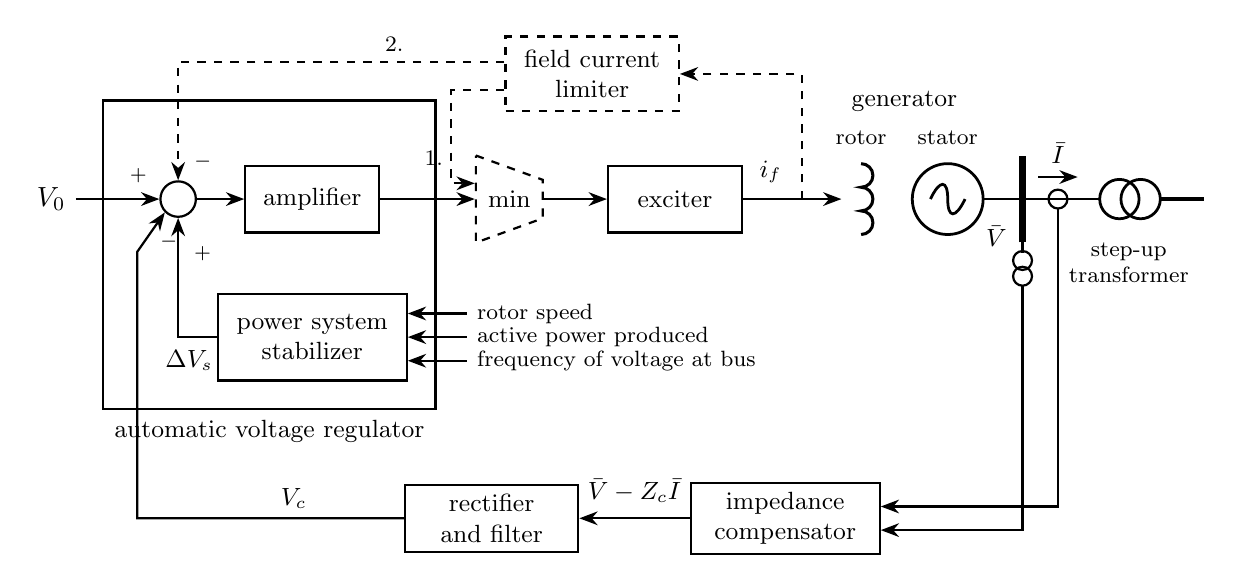
\begin{tikzpicture}[
    >=Stealth,
    line width=0.8pt,
    block/.style={draw, rectangle, minimum height=0.85cm, minimum width=1.7cm, align=center, font=\small},
    dashedblock/.style={draw, dashed, rectangle, minimum height=0.95cm, minimum width=2.2cm, align=center, font=\small},
    sum/.style={draw, circle, inner sep=0pt, minimum size=0.45cm}
]

% Summing junction & AVR inner blocks
\node[sum] (sum) at (0,0) {};
\node[block, right=0.6cm of sum] (amp) {amplifier};
\node[block, below=0.75cm of amp, minimum width=2.4cm, minimum height=1.1cm] (pss) {power system\\stabilizer};

% V0 input
\draw[->] (-1.3,0) node[left] {$V_0$} -- (sum.west) node[pos=0.75, above=2pt, font=\scriptsize] {$+$};

% Sum -> Amplifier
\draw[->] (sum.east) -- (amp.west);

% PSS -> Sum
\draw[->] (pss.west) -| (sum.south) node[pos=0.85, right=2pt, font=\scriptsize] {$+$};
\node[font=\small] at ($(pss.west)+(-0.35,-0.3)$) {$\Delta V_s$};

% PSS inputs
\draw[<-] ([yshift=0.3cm]pss.east) -- ++(0.75,0) node[right, font=\footnotesize] {rotor speed};
\draw[<-] (pss.east) -- ++(0.75,0) node[right, font=\footnotesize] {active power produced};
\draw[<-] ([yshift=-0.3cm]pss.east) -- ++(0.75,0) node[right, font=\footnotesize] {frequency of voltage at bus};

% AVR outer box
\coordinate (avr_tl) at (-0.6, 0.9);
\node[draw, fit=(sum) (amp) (pss) (avr_tl), inner sep=10pt, label={[below, font=\small]below:{automatic voltage regulator}}] (avrbox) {};

% Min block & Exciter
\node[draw, dashed, trapezium, trapezium angle=70, shape border rotate=270, minimum height=0.85cm, minimum width=0.75cm, right=1.2cm of amp, font=\small] (minblk) {min};
\node[block, right=0.8cm of minblk] (exc) {exciter};

% Field current limiter
\node[dashedblock, above=1.1cm of $(minblk)!0.5!(exc)$] (fcl) {field current\\limiter};

\draw[->] (amp.east) -- (minblk.west);
\draw[->] (minblk.east) -- (exc.west);

% Limiter dashed connections (1. and 2.)
\draw[->, dashed] ([yshift=-0.2cm]fcl.west) -| ([xshift=-0.3cm, yshift=0.2cm]minblk.west) -- ([yshift=0.2cm]minblk.west);
\node[font=\footnotesize] at ([xshift=-0.52cm, yshift=0.52cm]minblk.west) {1.};

\draw[->, dashed] ([yshift=0.15cm]fcl.west) -| (sum.north) node[pos=0.92, right=2pt, font=\scriptsize] {$-$};
\node[font=\footnotesize] at ($(fcl.west)+(-1.4,0.38)$) {2.};

% Exciter output -> Rotor -> Stator -> Bus -> Transformer
\coordinate (if_end) at ($(exc.east)+(1.25,0)$);
\draw[->] (exc.east) -- (if_end) node[pos=0.28, above=2pt, font=\small] {$i_f$};
\draw[->, dashed] ($(exc.east)+(0.75,0)$) |- (fcl.east);

% Rotor winding (3 arcs)
\begin{scope}[shift={($(if_end)+(0.25,0)$)}]
  \draw[line width=1.1pt] (0,0.45) arc (90:-90:0.15) arc (90:-90:0.15) arc (90:-90:0.15);
  \node[above=16pt, font=\footnotesize] at (0,0) {rotor};
\end{scope}

% Generator symbol
\coordinate (gen_c) at ($(if_end)+(1.35,0)$);
\draw[line width=1.0pt] (gen_c) circle (0.45);
\draw[line width=1.0pt] ($(gen_c)+(-0.22,0)$) .. controls ($(gen_c)+(-0.1,0.25)$) and ($(gen_c)+(0,0.25)$) .. (gen_c)
      .. controls ($(gen_c)+(0,-0.25)$) and ($(gen_c)+(0.1,-0.25)$) .. ($(gen_c)+(0.22,0)$);
\node[above=16pt, font=\footnotesize] at (gen_c) {stator};
\node[above=28pt, font=\small] at ($(if_end)+(0.8,0)$) {generator};

% Busbar & Step-up transformer
\coordinate (bus) at ($(gen_c)+(0.95,0)$);
\draw[line width=1.0pt] ($(gen_c)+(0.45,0)$) -- (bus);
\draw[line width=2.4pt] ($(bus)+(0,-0.55)$) -- ($(bus)+(0,0.55)$);
\node[below left=6pt and 2pt, font=\small] at (bus) {$\bar{V}$};

\coordinate (xfmr) at ($(bus)+(1.35,0)$);
\draw[line width=1.0pt] (bus) -- ($(xfmr)+(-0.35,0)$);
\draw[->, line width=0.8pt] ($(bus)+(0.2,0.28)$) -- ($(bus)+(0.7,0.28)$) node[midway, above=1pt, font=\small] {$\bar{I}$};
\draw[line width=1.0pt] ($(xfmr)+(-0.12,0)$) circle (0.25);
\draw[line width=1.0pt] ($(xfmr)+(0.15,0)$) circle (0.25);
\draw[line width=1.5pt] ($(xfmr)+(0.40,0)$) -- ($(xfmr)+(0.95,0)$);
\node[below=12pt, align=center, font=\footnotesize] at (xfmr) {step-up\\transformer};

% PT & CT measurement feedback
\node[block, below=3.15cm of exc, xshift=1.4cm, minimum width=2.4cm] (comp) {impedance\\compensator};
\node[block, left=1.4cm of comp, minimum width=2.2cm] (rect) {rectifier\\and filter};

% VT from bus
\coordinate (vt) at ($(bus)+(0,-0.9)$);
\draw (bus) -- ($(vt)+(0,0.22)$);
\draw ($(vt)+(0,0.12)$) circle (0.12);
\draw ($(vt)+(0,-0.08)$) circle (0.12);
\draw[->] ($(vt)+(0,-0.20)$) |- ([yshift=-0.15cm]comp.east);

% CT from line
\coordinate (ct_pos) at ($(bus)+(0.45,0)$);
\draw (ct_pos) circle (0.12);
\draw[->] ($(ct_pos)+(0,-0.12)$) |- ([yshift=0.15cm]comp.east);

% Compensator -> Rectifier -> Sum
\draw[->] (comp.west) -- (rect.east) node[midway, above=2pt, font=\small] {$\bar{V} - Z_c\bar{I}$};
\draw[->] (rect.west) -| ($(sum.south west)+(-0.35,-0.5)$) -- (sum.south west) node[pos=0.6, below right=-2pt, font=\scriptsize] {$-$};
\node[font=\small] at ($(rect.west)+(-1.4,0.25)$) {$V_c$};

\end{tikzpicture}
\end{document}
